\begin{multicols}{2}
\headline{Не преставайте да мечтаете}
\byline{Интервю с Елисавета Зайкова}{Венета, 12Е}

\noindent \begin{window}[2,r, 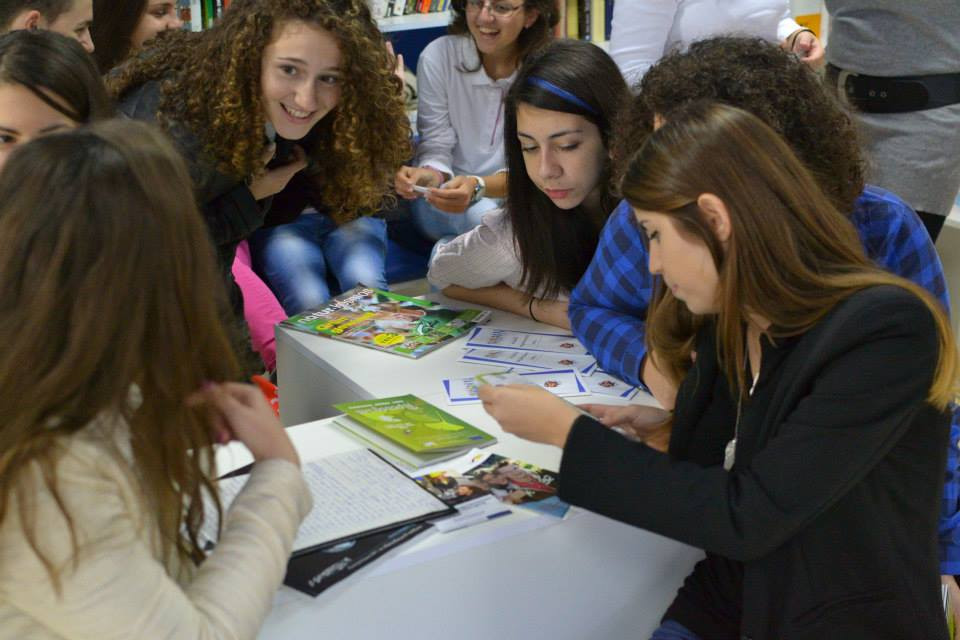
\includegraphics[width=3.4in]{./Zaikova/zaikova.jpg},] \end{window}

Какво най-много Ви допада в това да работите в Немската гимназия? 

Винаги е удоволствие да се работи с интелигентни и креативни млади хора, такива са учениците в гимназията. А и възрастта от 14 до 19 години е най-уязвимата и ранима възраст, изискваща силна подкрепа, разбиране и поощрение. Като добавим толерантността, целеустремеността, желанието да открият всички налични отговори и емоционалността на учениците, работата се превръща и в предизвикателство, и често в задача с повишена трудност, но може би затова ме привлича. 

С какви трудности сте се сблъсквали по време на работата си в Немската гимназия?

Честото отричане от страна на учениците - без алтернатива за промяна, без агрументация, само отхвърляне. В някои случаи и нежеланието да се положат взаимни усилия за постигането на обща цел. Тук учениците са най-вече индивидуалисти, всеки има своите невероятни качества, но изпитва известни съмнения и при формирането на екип. 

Какво можете да кажете за днешните ученици? 

Съвременните ученици са доста по-свободолюбиви, независими и борбени. Имат куража да се противопоставят и най-вече да следват своя път, да бъдат себе си! Много по-толерантни са и избягват стериотипи. Креативни са, по-искрени и с развито чувство за хумор и самоирония.

Пожелайте ни нещо по случай 55-годишнината на гимназията! 

Не преставайте да мечтаете, бъдете любознателни и търсещи.

\end{multicols}
